\section{High Application Layer CANae}
La denominada \textit{High Application Layer} tiene una función más del lado de
la gestión de nodos y tareas. En esta capa se desarrollan los algoritmos
necesarios para realizar el ruteo y la reconfiguración de la red ante fallas,
por lo tanto en la \textit{High Application Layer} se debe implementar la
\ac{FDIR}. El protocolo no define ninún algoritmo de ruteo, por lo que queda
para el usuario la definición de los algoritmos. Se recomienda desarrollar 2
algoritmos, el primario y el secundario. Para aumentar la tolerancia a fallas
se pueden desarrollar más algoritmos secundarios, y el switch entre algoritmos,
puede depender de medidas de perfomance.

En las Figuras [\ref{fig:HighAppLayerBlock}] y
[\ref{fig:HighAppLayerInternalBlock}] se pueden observar los diagramas de
bloques y diagramas de bloques internos para el \textit{High Application
Layer} de CANae. 

\begin{figure}[h!]
 \centering
 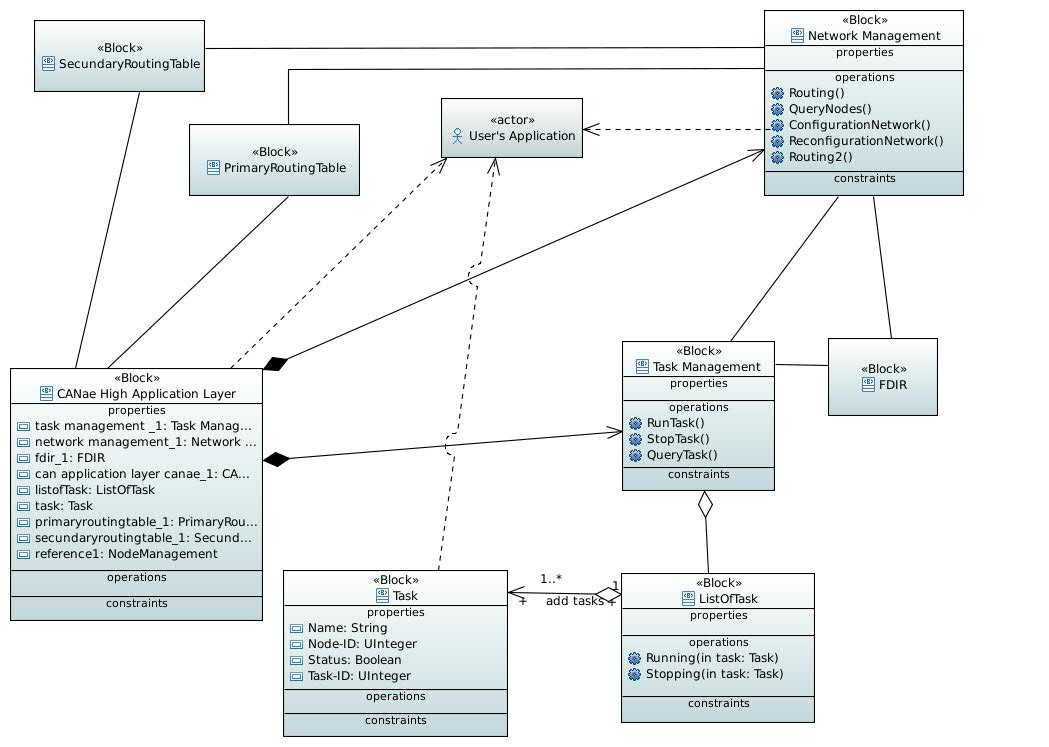
\includegraphics[scale=0.4]{images/Secciones/AppendixA/CANae_High_App_Layer.JPG}
  \caption{Diagrama de bloques del High Application Layer de CANae}
\label{fig:HighAppLayerBlock}
\end{figure}

\begin{figure}[h!]
 \centering
 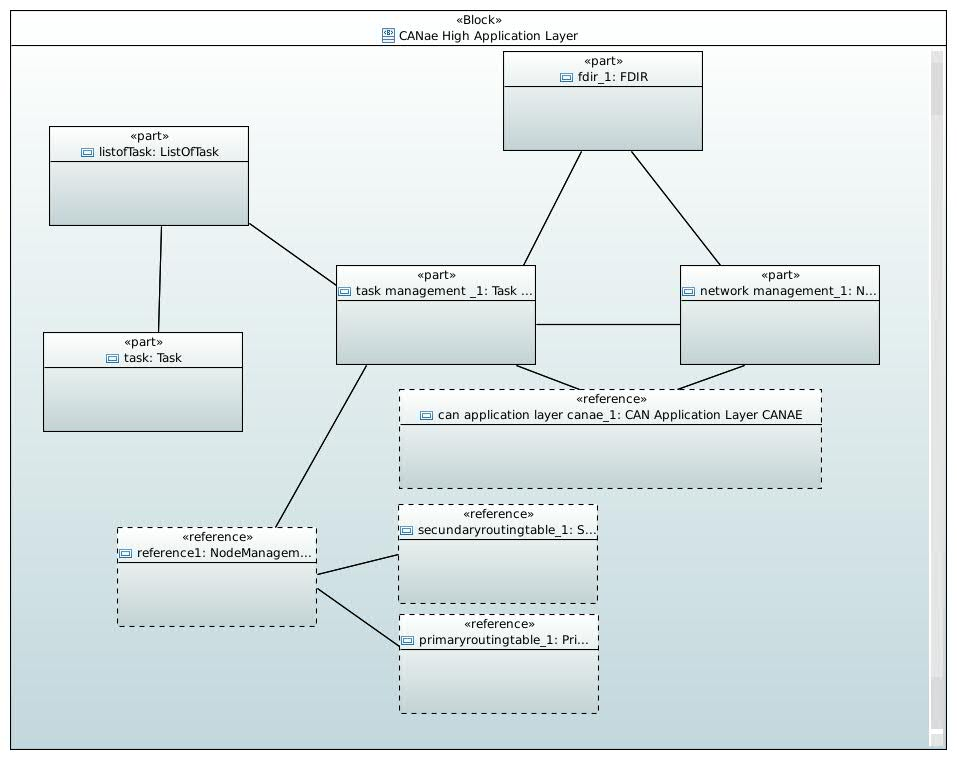
\includegraphics[scale=0.4]{images/Secciones/AppendixA/Internal_CAN_High_Application_Layer.JPG}
  \caption{Diagrama de bloques internos del High Application Layer de CANae}
\label{fig:HighAppLayerInternalBlock}
\end{figure}

Esta capa está compuesta por varias entidades, las cuales tienen solo una
instancia por entidad.

En la \textit{High Application layer} se encuentra la entidad más importante, la
cual es el \ac{FDIR}. El desarrollo de esta entidad se encuentra fuera del
alcance de esta versión (0.1 Alpha) del protocolo.

\subsection{Network Management}
Esta entidad se encarga de la gestión de la red desde el punto de vista del
nodo. La entidad utiliza el \textit{NodeTableConfiguration} del
\textit{CANae Application Layer}.

Los servicios brindados por el \textit{Network Management} son los siguientes:
\begin{itemize}
\item \textbf{Routing()}: este servicio lleva a cabo el ruteo de los mensajes.
  Este servicio consulta la tabla \textit{NodeTableConfiguration}.
\item \textbf{QueryNodes()}: este servicio hace consulta de los nodos
  conectados. Este puede ser utilizado por el servicio Routing()
\item \textbf{ConfigurationNetwork()}: este servicio se lleva a cabo solo una
  vez, durante el encendido y configuración al nodo. 
\item \textbf{ReconfigurationNetwork()}: este servicio lleva a cabo la
  reconfiguración de la red. Este servicio es activado por el \ac{FDIR} una vez
  que detecta algún error.
\item \textbf{Routing2()}: Este servicio se lleva a cabo cuando se detecta un
  error en la red. Lo activa el \ac{FDIR}. 
\end{itemize}

El comportamiento del \textit{Network Management} es sencillo, cuando se
enciende por primera vez el nodo, de manera automática, la aplicación de
usuario debe llamar el servicio \textit{ConfigurationNetwork()} al \textit{
  Network Management} esta entidad se comunica con el \textit{Node Management}
para que se genere la ``Tabla Primaria de Ruteo''. Una vez que esta
tabla se encuentre generada (tal como se hace referencia en
\ref{subsection:tablaprimariaysecundaria}), la aplicación de usuario puede enviar señales
de \textit{QueryNodes()} y \textit{Routing()}. Esto se puede ver visualmente en
la Figura \ref{fig:NetworkManagementInteration}.

\begin{figure}[h!]
 \centering
 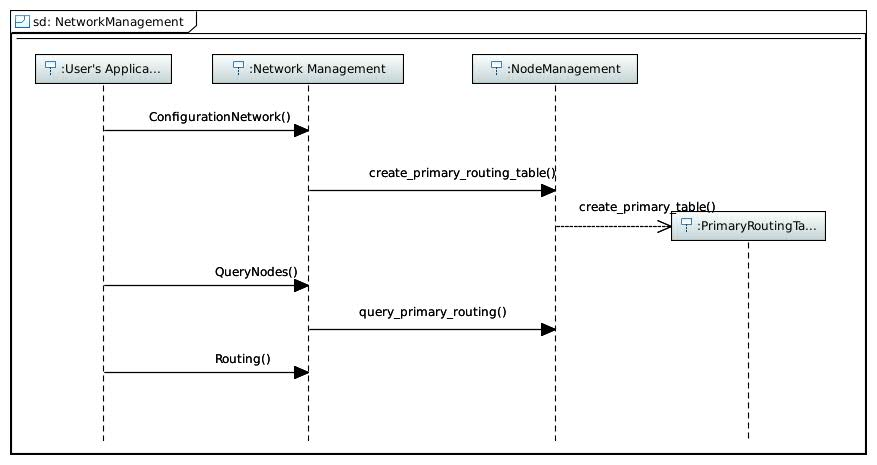
\includegraphics[scale=0.4]{images/Secciones/AppendixA/NewtworkManagement.JPG}
 \caption{Diagrama de interacción del comportamiento del \textit{Network
 Management}}
\label{fig:NetworkManagementInteration}
\end{figure}

En caso de errores, esto debe ser captado por el \ac{FDIR} del sistema. El
comportamiento del mismo se muestra en la Figura
\ref{fig:NetworkManagementInterationError}

\begin{figure}[h!]
 \centering
 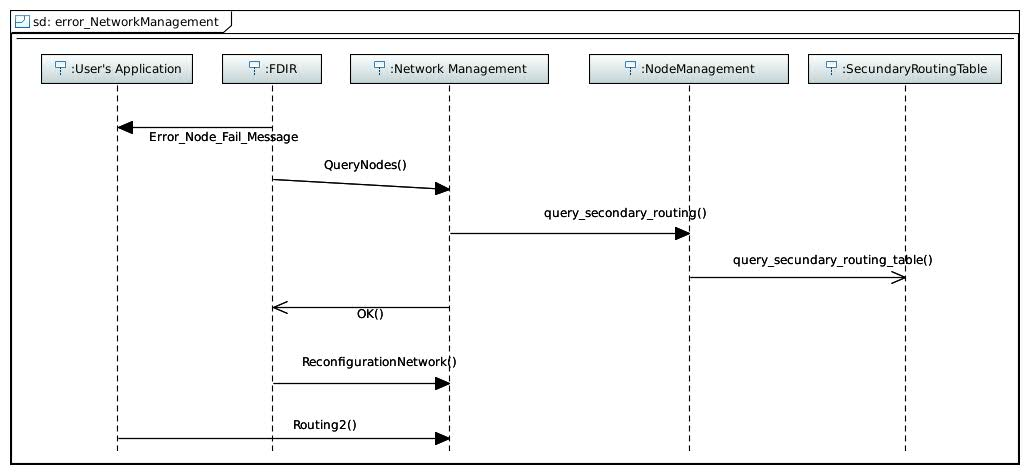
\includegraphics[scale=0.4]{images/Secciones/AppendixA/errorNetworkmanagement.JPG}
 \caption{Diagrama de interacción del comportamiento del \textit{Network
     Management en caso de errores}}
\label{fig:NetworkManagementInterationError}
\end{figure}

\subsection{Task Management}
Esta entidad se encarga de la gestión de las tareas. Debe aclararse que esta es
una abstracción, y no depende del Sistema Operativo que se utilice para la
codificación del sistema. El objetivo de esta entidad es mantener la
distribución de las tareas entre los nodos de la red. Esto permitiría que cuando
deja de funcionar (detectado por el \ac{FDIR}) uno de los nodos, el
\textit{Task Management} gestiona las tareas que se desarrollan en los nodos.
Para ellos se hace uso de la ``Lista de Tareas'' (\textit{ListOfTask}).
 
Los servicios que ofrece el \textit{Task Management} son los siguientes:
\begin{itemize}
\item \textbf{RunTask()}: este servicio activa las tareas para ejecutarse en
  el nodo.
\item \textbf{StopTask()}: este servicio detiene las tareas que se ejecutan en
  el nodo.
\item \textbf{QueryTask()}; este servicio hace consulta de las tareas que
  existene la ``lista de Tareas''.
\end{itemize}

El comportamiento de esta entidad es sencilla. La aplicación de usuario le envía
una señal de \textit{QueryTasks()} con el motivo de conocer todas las tareas que
se están ejecutando en la red. El \textit{Task Management} lleva a cabo un
\textit{query\_tasks\_in\_network()} al \textit{Network Management} el cual le
provee la información. La primera comprobación que debe realizar la
aplicación de usuario es que la tarea no existe en otro nodo ejecutandose. Luego
de esta comprobación ya tiene permitido llevar a cabo el \textit{RunTask()}. Por
último el \textit{Task Management} manda el mensaje \textit{Running(Task task)}
al \textit{ListOfTasks}(ver \ref{subsection:listoftask}). El comportamiento de
la entidad se la puede observar en la Figura \ref{fig:TaskManagement_RunTask}.

\begin{figure}[h!]
 \centering
 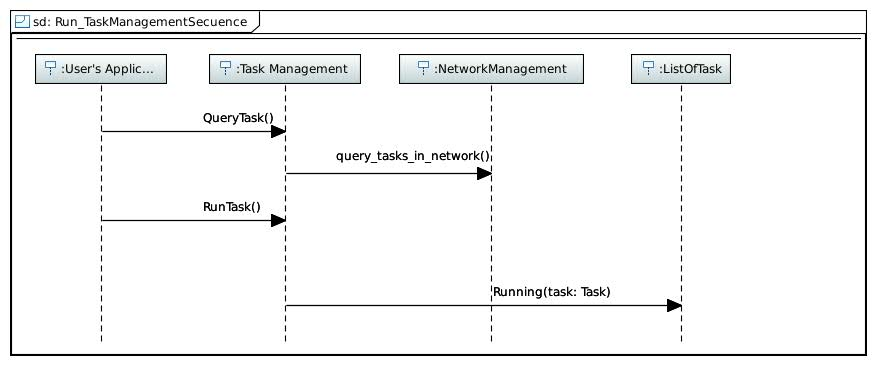
\includegraphics[scale=0.4]{images/Secciones/AppendixA/TaskManagement.JPG}
  \caption{Diagrama de secuencia de la ejecución de tareas del Task Management}
\label{fig:TaskManagement_RunTask}
\end{figure}

Por otro lado cuando la aplicación de usuario necesita para una tarea, o debido
a que el FDIR detecto una falla y necesita detener la ejecución de una tarea, el
proceso que debe llevar el \textit{Task Management} es el siguiente, en primer
hace un \textit{QueryTasks()} para conocer las tareas que se están ejecutando y
sus estados. Luego manda un señal de \textit{StopTask()} al \textit{Task
  Management}. Esta, envía mensajes de \textit{query\_tasks\_in\_network()},
y luego el \textit{Stopping(Task task)} para detener la ejecución del proceso.
En la Figura \ref{fig:TaskManagement_StopTask}

\begin{figure}[h!]
 \centering
 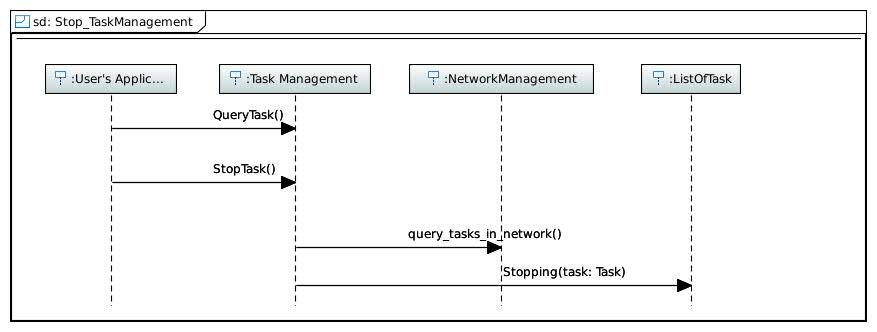
\includegraphics[scale=0.4]{images/Secciones/AppendixA/Stop_TaskManagement.JPG}
 \caption{Diagrama de secuencia para detener procesos por parte del
   Task Management}
\label{fig:TaskManagement_StopTask}
\end{figure}

\subsection{List of Tasks}\label{subsection:listoftask}
Este es un objeto que mantiene una lista de las tareas que se están definidas en
el sistema. Estas tareas pueden o no estar ejecutandose. Esta lista tiene un
instancia a todas las tareas. 

Los servicios que se ejecutan en esta entidad son los siguientes:
\begin{itemize}
\item \textbf{Running(Task task)}: este servicio ejecuta una tarea.
  \begin{itemize}
    \item \textbf{Task task}: tarea a ejecutar.
  \end{itemize}  
\item \textbf{Stopping(Task task)}: este servicio detiene una tarea.
  \begin{itemize}
    \item \textbf{Task task}: tarea a ejecutar.
  \end{itemize}
\end{itemize}

\subsection{Task}
Este es un objecto que representa la abstracción de las tareas. Las propiedades
de esta entidad son las siguientes:
\begin{itemize}
\item \textbf{String Name}: es el nombre de la tarea.
  \item \textbf{UInteger Task-ID}: es el ID de la tarea.
  \item \textbf{UIntenger Node-ID}: es el ID del nodo donde se está ejecutando
    la tarea.
  \item \textbf{Boolean Status}: es el status de la tarea \{RUNNING, STOPED\}
\end{itemize}



